\section{Half-precision floating-point numbers}
A significant performance improvement was achieved by transitioning from single-precision floating-point numbers to half-precision floating-point numbers.
Half-precision floating-point numbers are 16-bit floating-point numbers with 11 bits of significand precision, which adequately accommodate the 10-bit pixel values \cite{HalfprecisionFloatingpointFormat2023}.
The utilization of half precision floating-point numbers yield notable gains due to the dedicated hardware present in the \gls{gpu}s \gls{alu} \cite{CUDA2023}.
\footnote{This should not be confused with Tensor cores, which also operate on half-precision floating-point numbers but are not employed in this project}.
This dedicated hardware allows for \gls{simd} operations on a specialized data format called \code{__half2} \cite{nvidiaHalf2ArithmeticFunctions2023}.

This is particularly useful in this context, as each row costist of alternating polarization channels, which can be transformet to the \code{__half2} format, as shown in Listing \ref{listing:generated_function}, and the processed in parallel.
This is visualized in Figure \ref{fig:half2_conv}.

\begin{figure}[H]
    \centering
    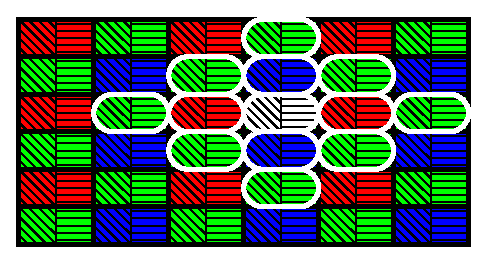
\includegraphics[width=0.45\textwidth]{figures/polarized_image/half2_conv.pdf}
    \caption{Vusialization of the convolution performed on the \code{__half2} data type. The pairs of pixels encircled are stored in a single \code{__half2} variable.}
    \label{fig:half2_conv}
\end{figure}

The main disadvantage of using \code{__half2} arithmetic is that every operation even addition, as to be performed using a function call \cite{nvidiaHalf2ArithmeticFunctions2023}
Fortunately this was not a big issue in this case, as the arithmetic operations are generated by the \py script,discussed in Section \todo, which could be modified to generate the correct function calls as shown in Listing \ref{listing:generated_function}.


\subsection{Small Infinities}

Half-precision floating points consider any value exceeding $65504$ as infinity \cite{HalfprecisionFloatingpointFormat2023}.
This can pose a problem when performing calculations that might exceed this threshold during intermediate steps, resulting in the value being treated as infinity.
In the preprocessing phase, this issue occasionally arises since the \code{P010_10LE} format utilizes the 10 most significant bits of a 16-bit integer, approaching the limit of half-precision floating points.

This was particularly problematic when the resulting values were cast to integers, as the resulting value would be zero, causing unexpected black spots in the image.
To mitigate this problem, the floating-point values are now cast to integers within the range of 0 to 1023, followed by a left bitshift of 6 bits to conform to the \code{P010_10LE} format.


